\documentclass[10pt]{article}
\usepackage{geometry}                % See geometry.pdf to learn the layout options. There are lots.
\geometry{letterpaper}                   % ... or a4paper or a5paper or ... 
\usepackage{graphicx}			% insertar gráficos
\usepackage{amssymb}			% Símbolos
\usepackage{hyperref}			% para incluir hiper-referencias
\usepackage{titlesec}			% Cambiar formato de títulos
\usepackage[plain, noabstract, nocomment]{flexbib} % Para citar con paréntesis y cosas así 
% https://www.nacho-alvarez.es/index.php/blog/2007/04/15/estilo-de-bibliografia-para-bibtex/
% http://www.latex.um.es/retazos/leccion_15/flexbib_manual.pdf
% Editato el spanishbst.tex y flexbib.sty
\usepackage{appendix} % Anexos
\usepackage{placeins}
\usepackage{scrextend}
\usepackage{fontspec,xltxtra,xunicode}		% Por defecto
\usepackage{subcaption}
\defaultfontfeatures{Mapping=tex-text}		% Para usar Century Gothic
\setmainfont[		% Para usar Century Gothic
 BoldFont={Century Gothic Bold}, 
 ItalicFont={Century Gothic Italic},
 BoldItalicFont={Century Gothic Bold Italic}
 ]{Century Gothic}

\addtokomafont{labelinglabel}{\sffamily}

\bibpunct{(}{)}{;}{a}{,}{,} % Modificar como se cita https://en.wikibooks.org/wiki/LaTeX/Bibliography_Management

\renewcommand{\bibsection}{\section{Bibliografía\\}} % Cambiar nombre de la bibliografía insertada al final del documento
\renewcommand{\figurename}{Figura} % Cambiar el nombre de las figuras
\renewcommand{\tablename}{Cuadro} % Cambiar el nombre de las tablas
\renewcommand{\contentsname}{Tabla de contenidos\\} % Cambiar el nombre de la tabla de contenidos
\renewcommand{\listfigurename}{Índice de figuras\\} % lista de figuras
\renewcommand{\listtablename}{Índice de cuadros\\} % lista de cuadros
%http://www.elmundoenbits.com/2012/03/latex-problemas-con-el-anexos.html#.WOrWdVKZNE4
\renewcommand{\appendixname}{Anexos}
\renewcommand{\appendixtocname}{Anexos}
\renewcommand{\appendixpagename}{Anexos}

\setlength{\parindent}{0pt}

\titleformat*{\section}{\normalsize\bfseries}
\titleformat*{\subsection}{\normalsize\bfseries}
\titleformat*{\subsubsection}{\normalsize\bfseries}

\title{Tutorial uso de GitHub Desktop}
\author{Aldo Tapia}
%\date{}                                           % Activate to display a given date or no date

\begin{document}
\maketitle

\textbf{Git} es un sistema de control de versiones de código abierto. El objetivo de su uso es poseer un seguimiento de los cambios realizados sobre un archivo y fomentar el trabajo colaborativo. Por otro lado, \textbf{GitHub} es una plataforma para alojar proyectos desarrollados en Git y facilitar su uso. Git funciona mediante líneas de comando, mientras que GitHub funciona con una interfaz gráfica en la web o en escritorio.\\

Ya que latex es un lenguaje de programación, la utilización de GitHub es ideal el control de versiones y corrección de documentos de manera colaborativa.\\

\section{Configuración GitHub Desktop}

El primer paso es descargar \textbf{GitHub Desktop} desde la página web \url{https://desktop.github.com/} (Figura \ref{desktop}). Luego de la instalación, crear una cuenta en \url{https://github.com/} (Figura \ref{web}) y añadir la cuenta a GitHub Desktop (Figura \ref{cuenta}).\\

\begin{figure}[!h]
  \centering
    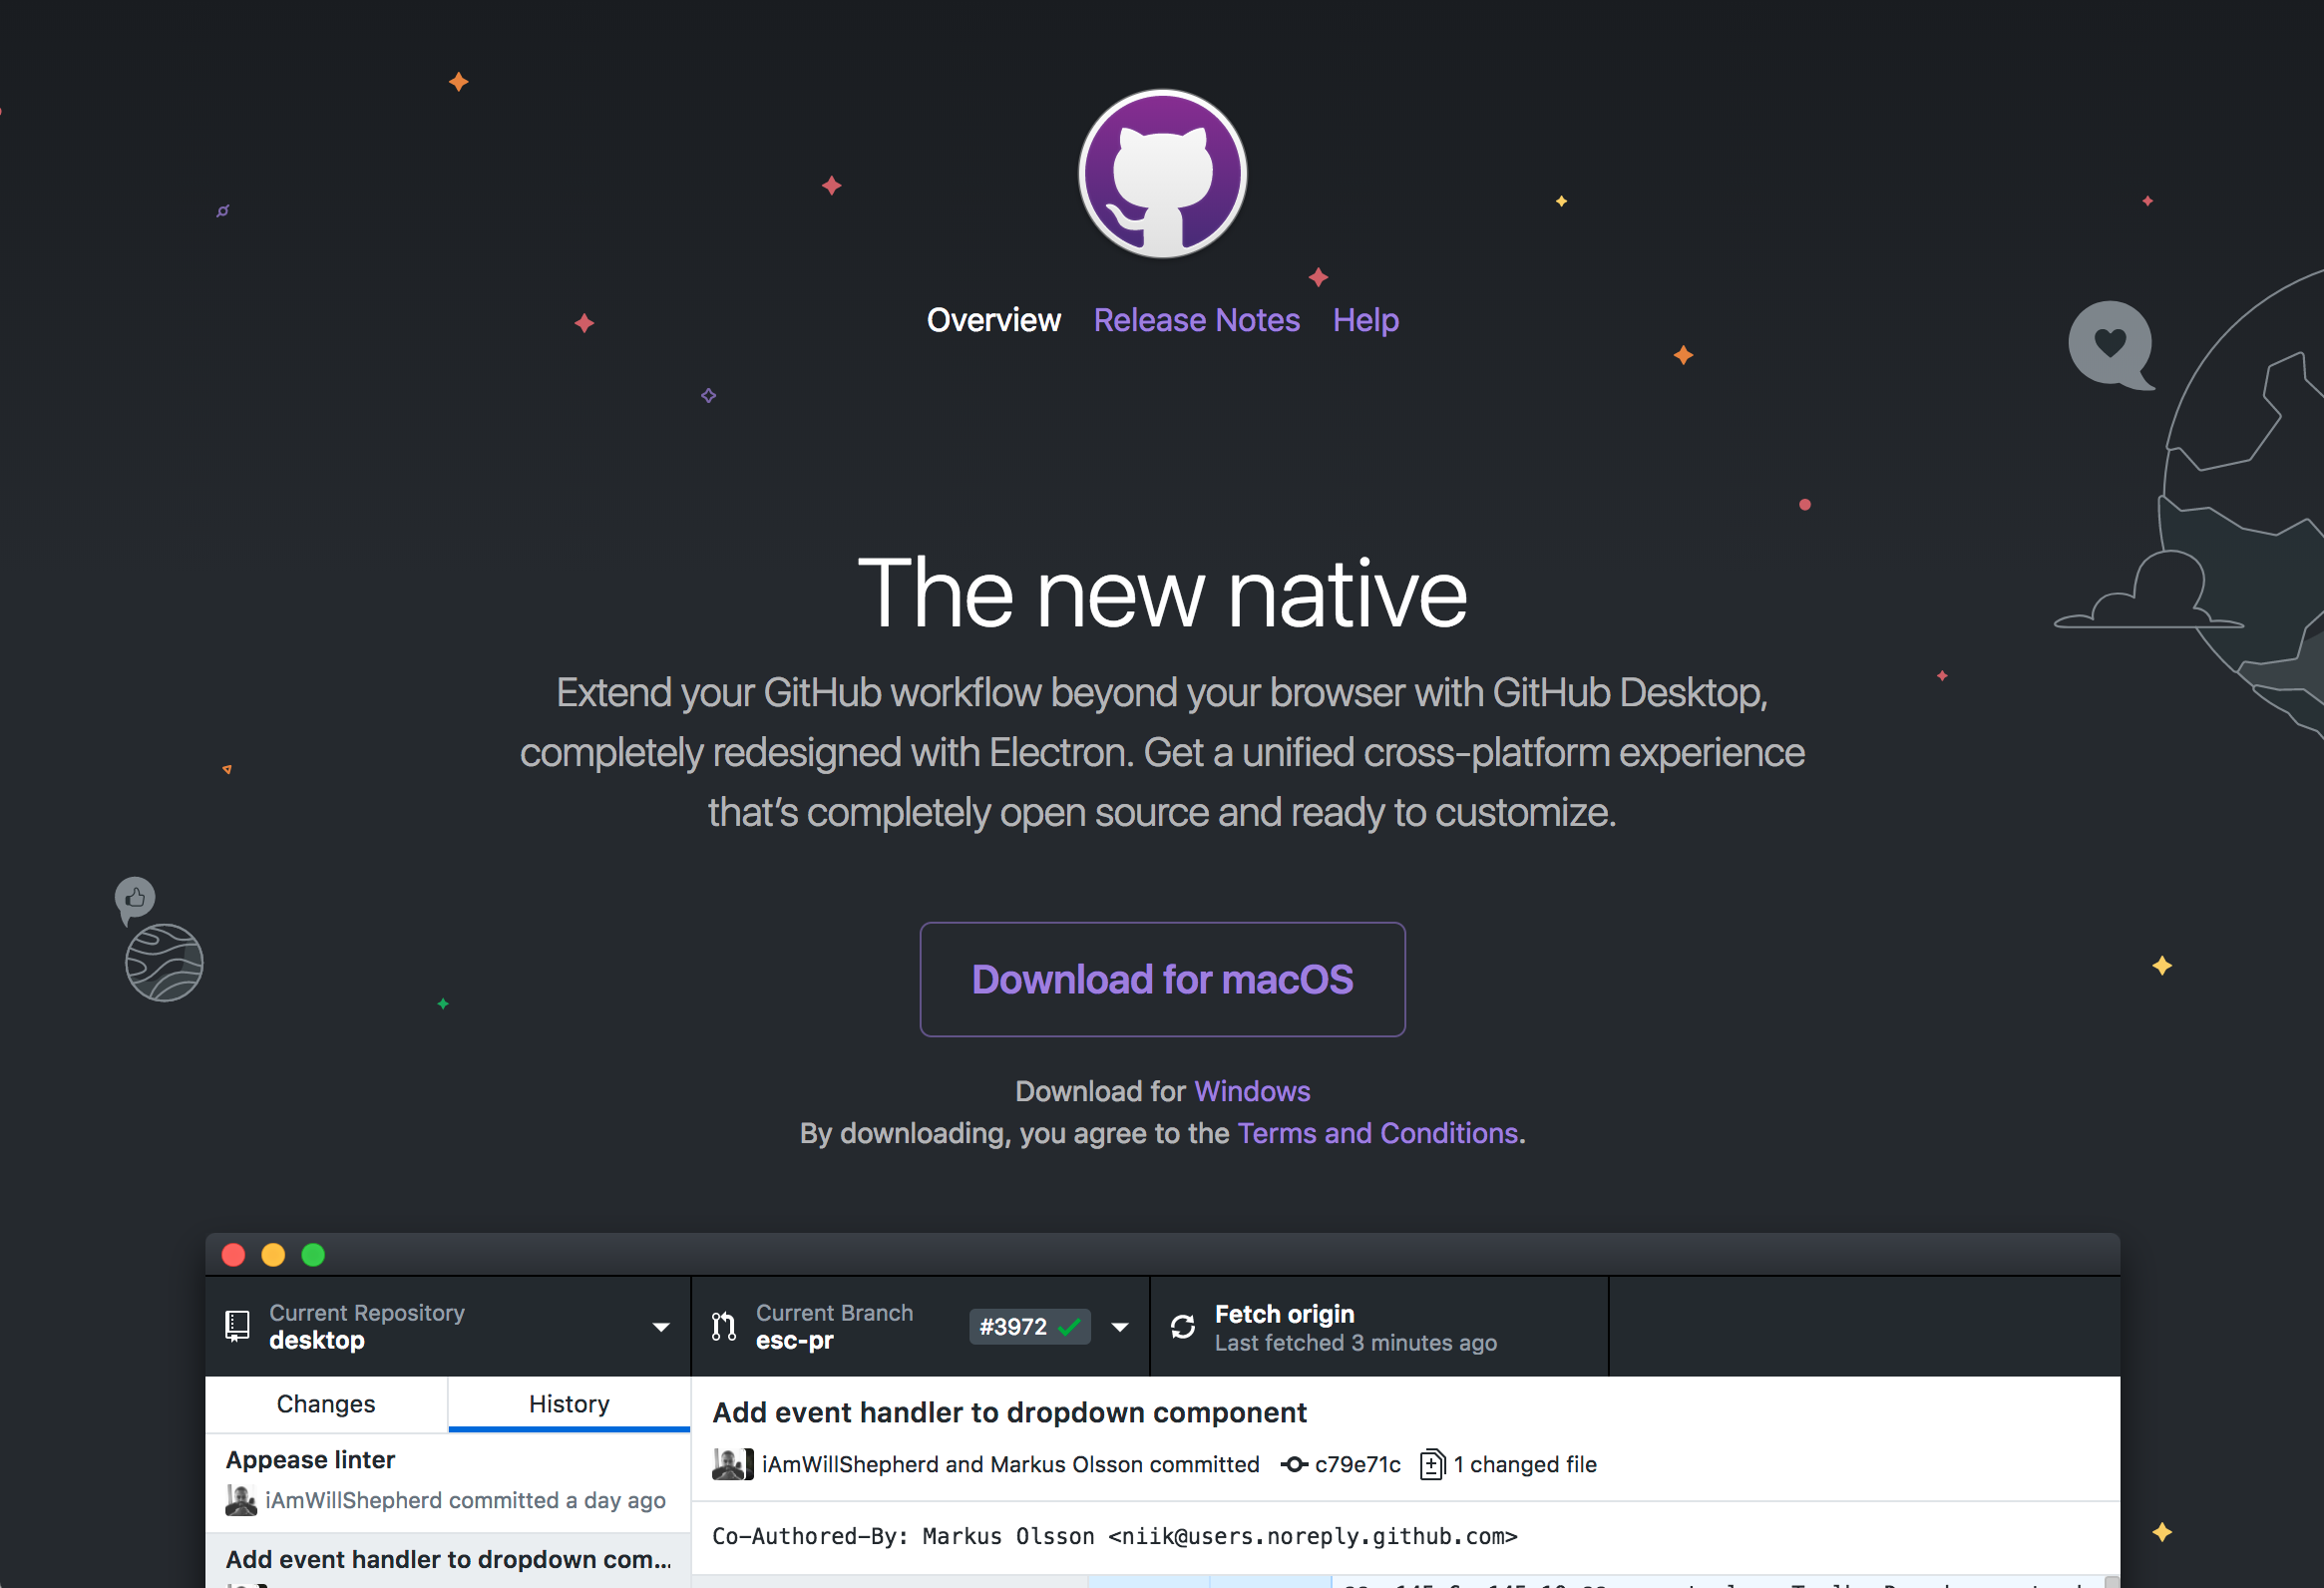
\includegraphics[width=0.5\textwidth]{Figuras/desktop.png}
  \caption{Página web de descarga de GitHub Desktop.}
  \label{desktop}
\end{figure}

\begin{figure}[!h]
  \centering
    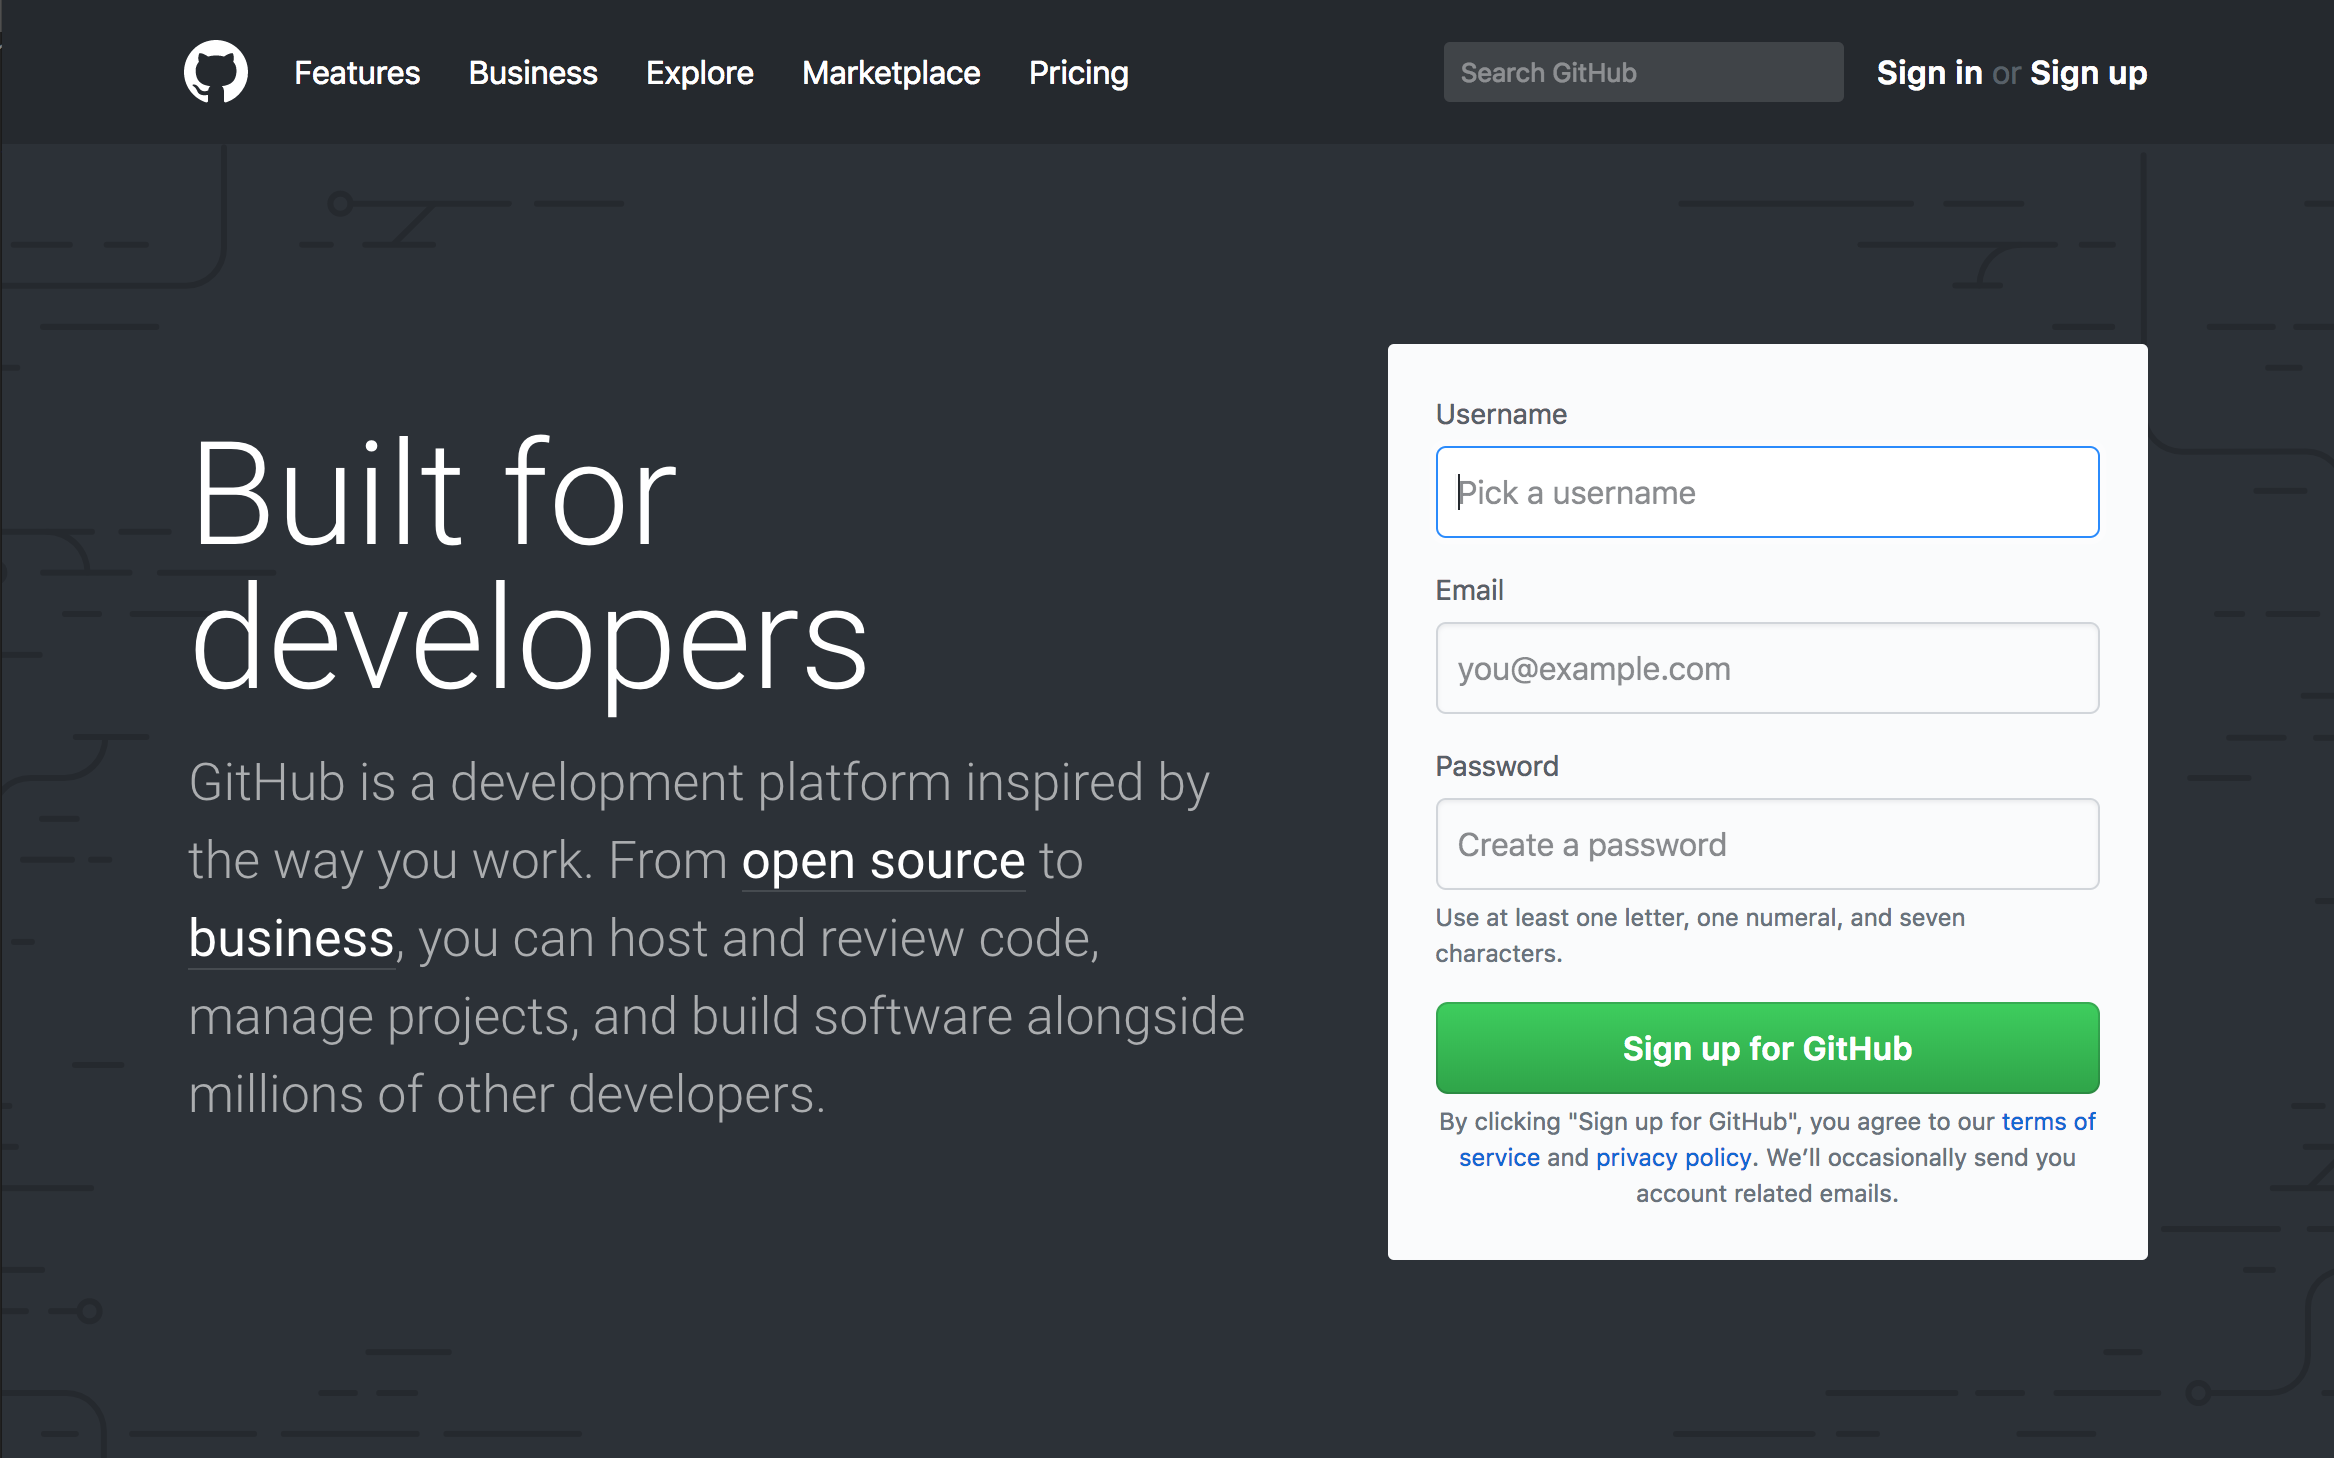
\includegraphics[width=0.5\textwidth]{Figuras/web.png}
  \caption{Creación de cuenta en GitHub.}
  \label{web}
\end{figure}

\begin{figure}[!h]
  \centering
    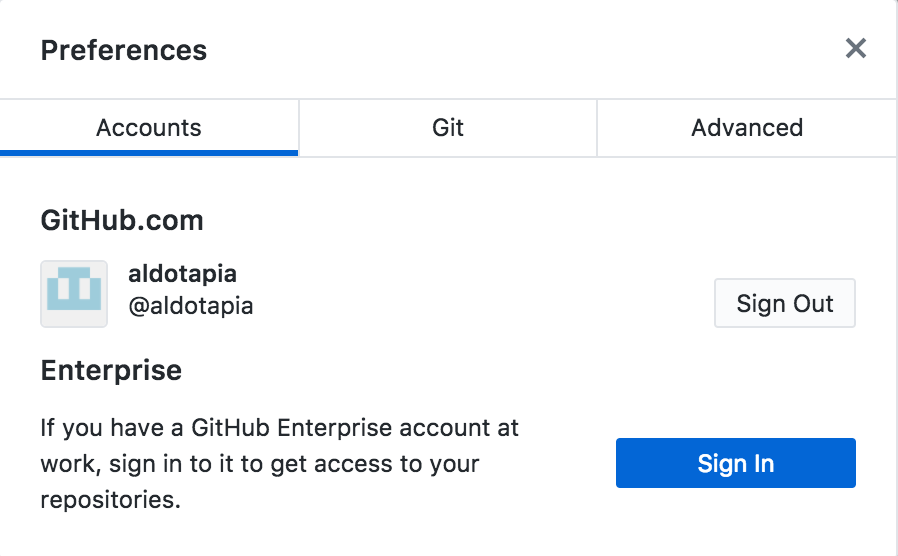
\includegraphics[width=0.5\textwidth]{Figuras/cuenta.png}
  \caption{Configuración de cuenta en GitHub Desktop.}
  \label{cuenta}
\end{figure}

\FloatBarrier

\section{Funcionamiento básico}

\textbf{Crear un repositorio}: Un repositorio es una suerte de proyecto, en el cual se van añadiendo los archivos. Cada versión considera todos los cambios realizados en un mismo repositorio. Para crearlo ir a \texttt{File/New Repository}. Las opciones son las que aparecen en la Figura \ref{repo}. Las opciones son las siguientes:\\

\begin{labeling}{elerepo}
\item [Name] Nombre del repositorio.
\item [Description] Descripción del repositorio.
\item [Local Path] Ruta donde se almacenan los archivos.
\item [Selección] ¿Incluir archivo \textbf{README} en la carpeta?
\item [Git Ignore] Extensión de archivos a ignorar por defecto.
\item [License] Tipo de licencia (None).
\end{labeling}

\begin{figure}[!h]
  \centering
    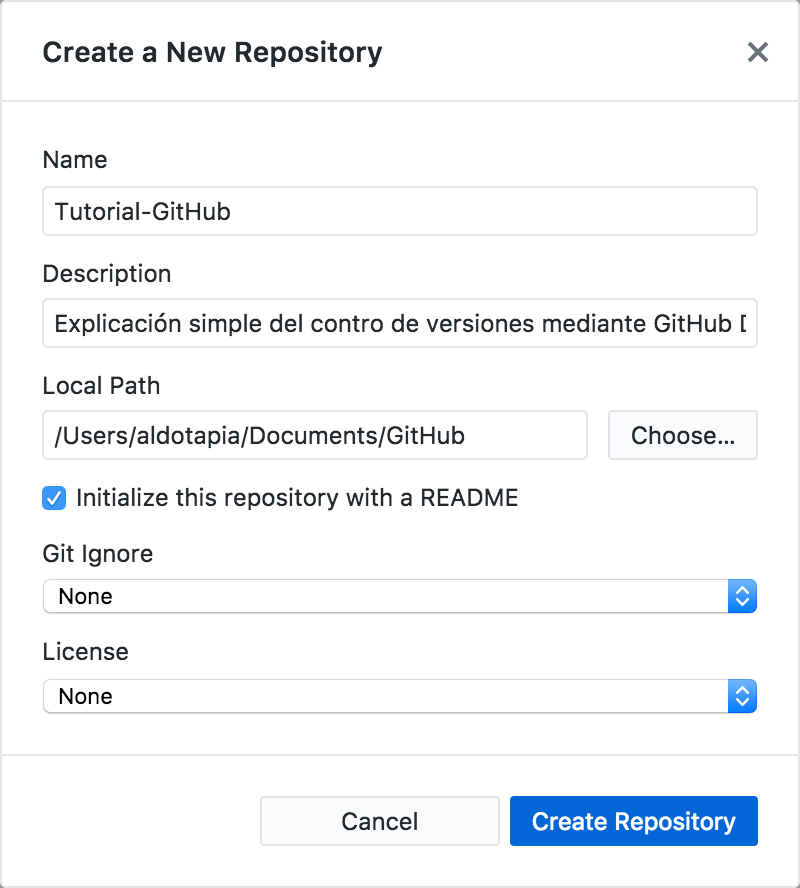
\includegraphics[width=0.3\textwidth]{Figuras/repo.png}
  \caption{Crear nuevo repositorio.}
  \label{repo}
\end{figure}

\FloatBarrier

\textbf{Añadir archivos}: Para añadir los primeros archivos al repositorio, simplemente moverlos a la carpeta del repositorio. Estos aparecerán en GitHub Desktop con un símbolo [+] (Figura \ref{archivos}).\\

\begin{figure}[!h]
  \centering
    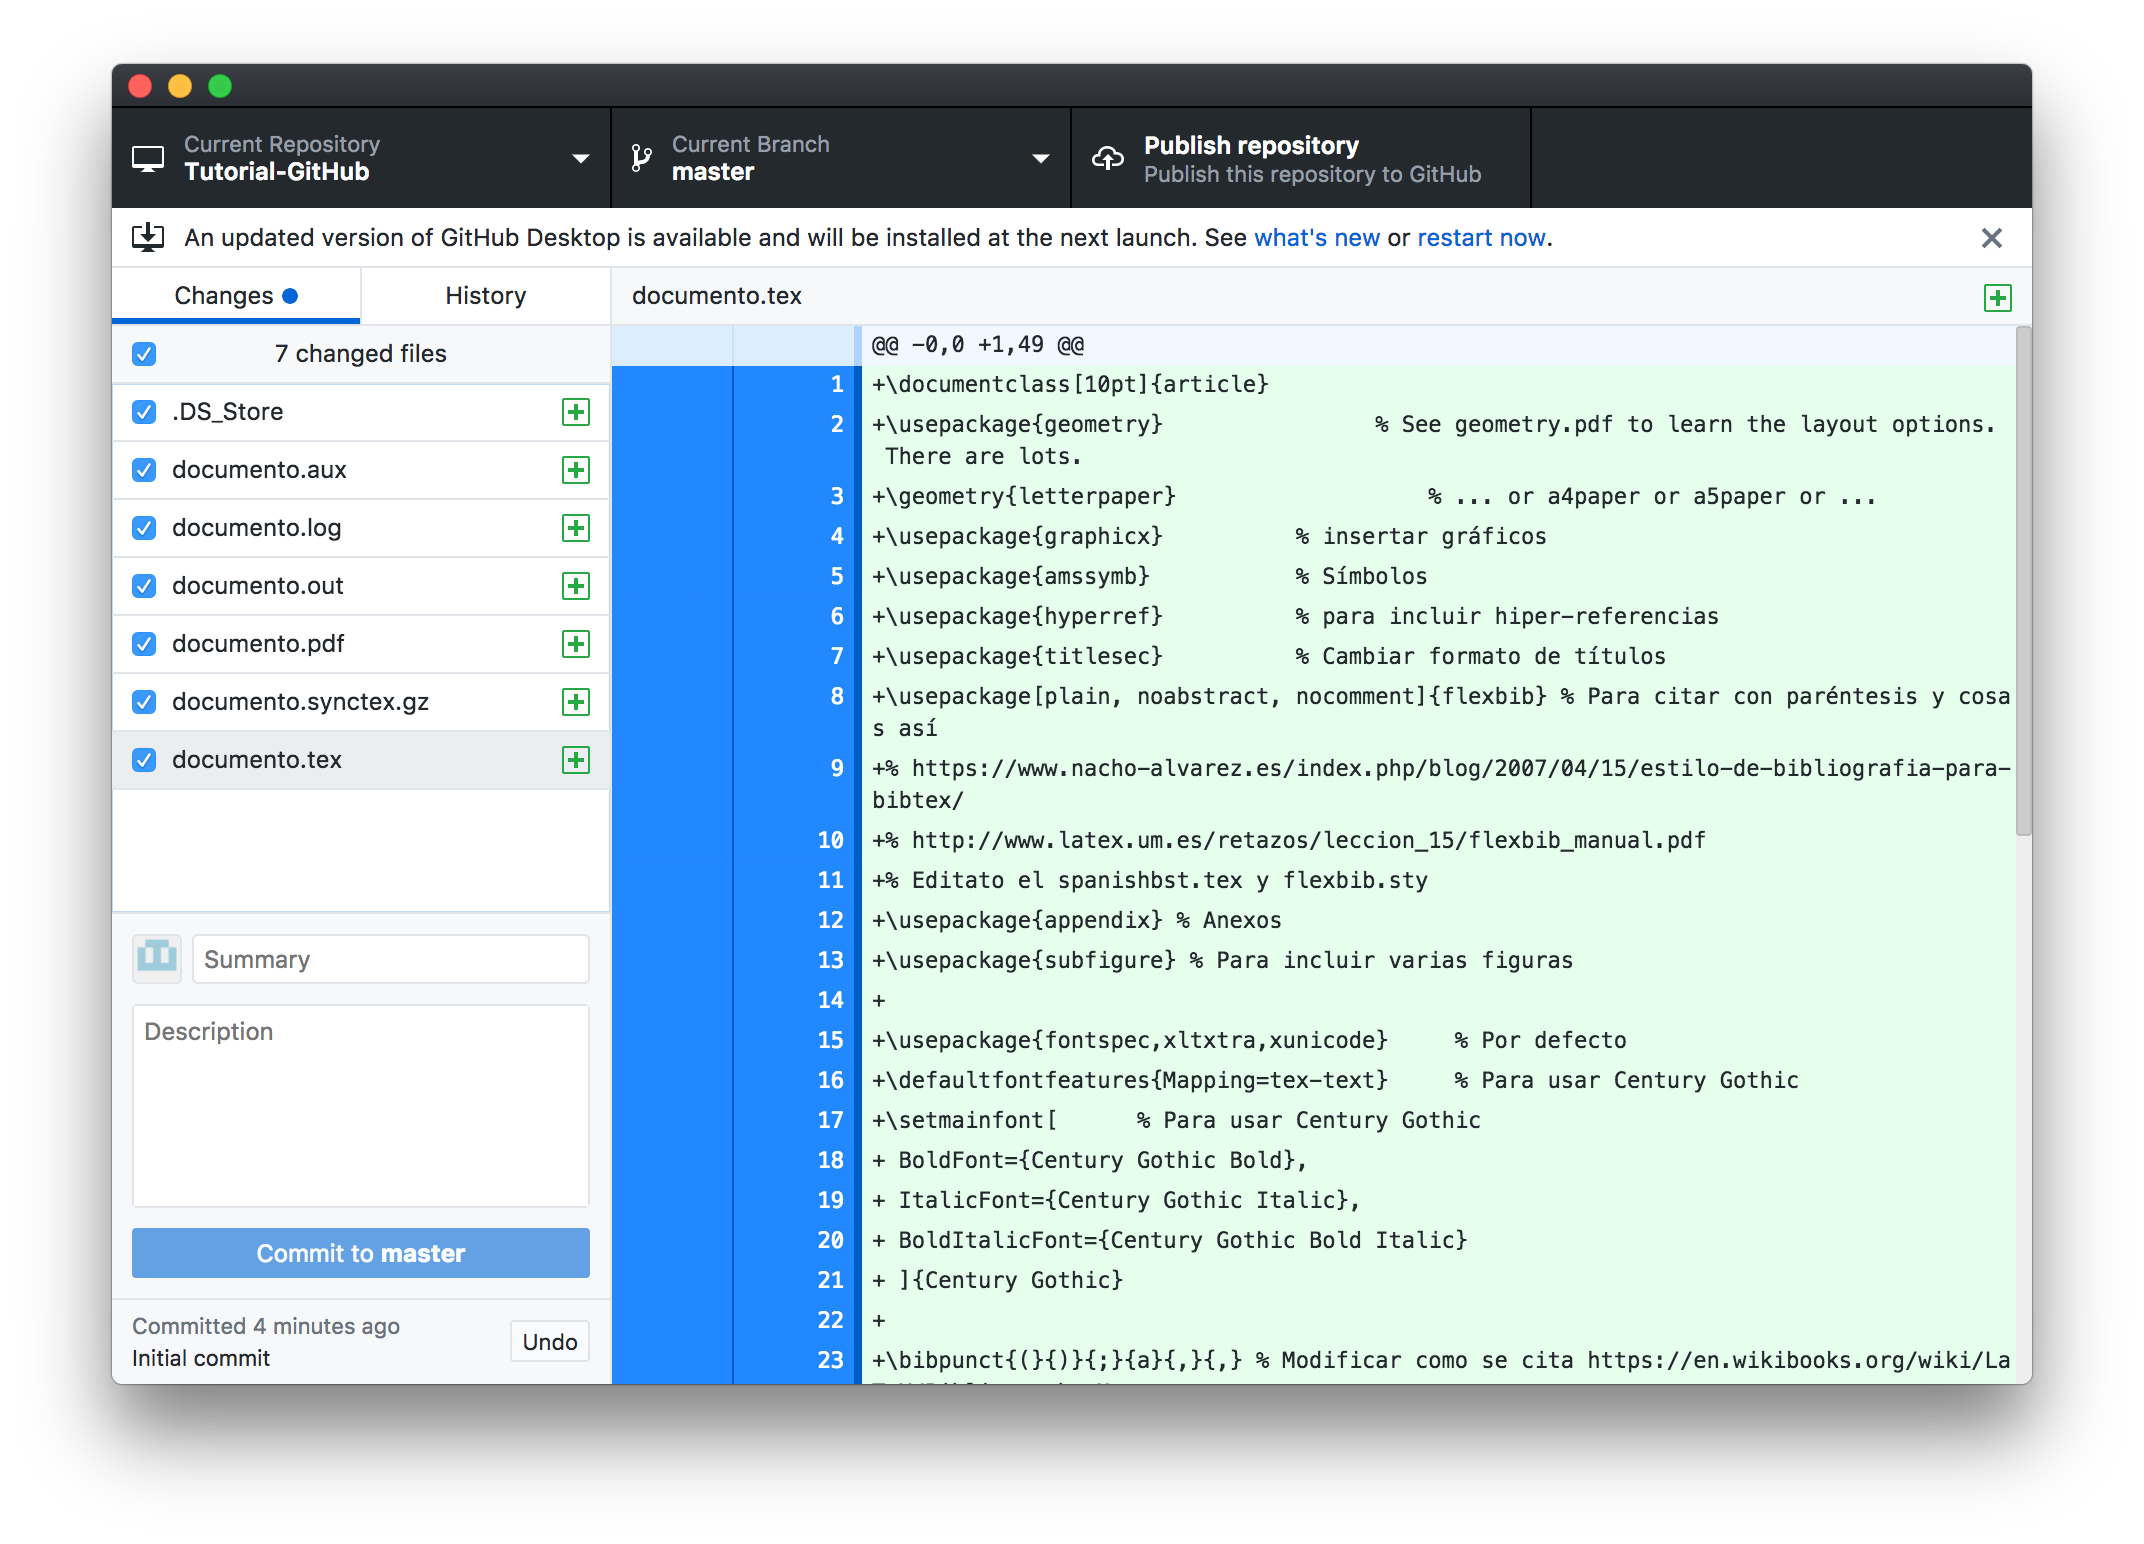
\includegraphics[width=0.5\textwidth]{Figuras/archivos.png}
  \caption{Crear nuevo repositorio.}
  \label{archivos}
\end{figure}

En la Figura \ref{archivos}, sobre el texto en verde, aparece \texttt{@@ -0,0 +1,49 @@}, lo que significa que no se ha eliminado ninguna línea (\texttt{-0,0}) y que se han añadido líneas, desde la linea 1, un total de 49 líneas (\texttt{+1,49}). Esto es útil para saber rápidamente los cambios que se han producido entre documentos.\\

La acción de añadir versiones de archivos se denomina \texttt{Commit}. Cada \texttt{Commit} guarda una versión de todos los archivos en los cuales ha habido cambios (los cuales son visibles en la pestaña \textbf{Changes}). Quizás no todos los archivos que se encuentran dentro de la carpeta es necesario incluirlos en el \texttt{Commit}, para ello simplemente se deseleccionan, dejando seleccionados sólo los archivos que se pretenden añadir al \texttt{Commit}. Se debe incluir un resumen y descripción del \texttt{Commit} y luego clickear \texttt{Commit to \textbf{master}} (Figura \ref{cambios1}), siendo \textbf{master} la rama por defecto del repositorio (revisar  \url{http://rogerdudler.github.io/git-guide/index.es.html} para más detalles de ramas o el funcionamiento de Git). Una vez hecho el \texttt{Commit}, desaparecerán los archivos añadidos, ya que los cambios que existían han sido incluidos en la actual rama (Figura \ref{cambios2}).\\

\begin{figure}[!h]
    \centering
    \begin{subfigure}[b]{0.3\textwidth}
        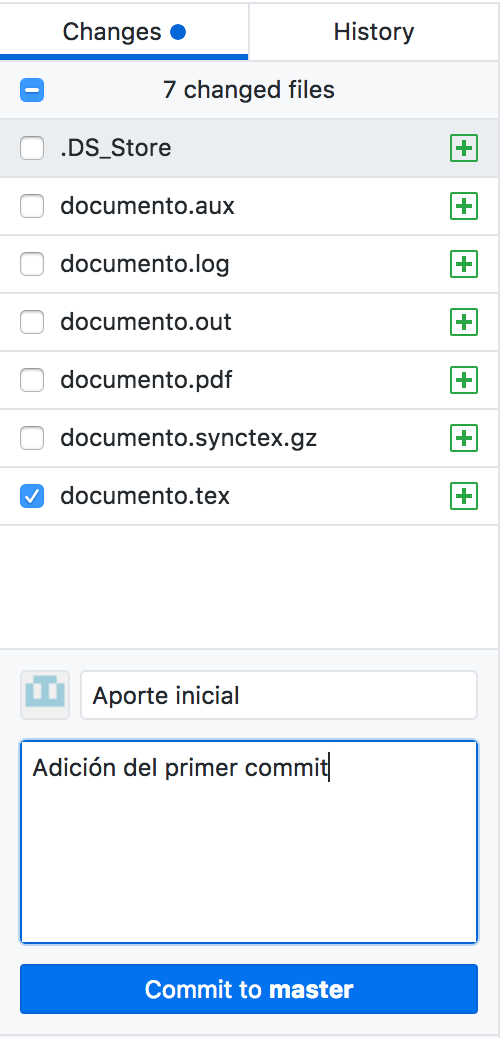
\includegraphics[width=\textwidth]{Figuras/cambios1.png}
        \caption{Antes de \texttt{commit}.}
        \label{cambios1}
    \end{subfigure}
    ~ %add desired spacing between images, e. g. ~, \quad, \qquad, \hfill etc. 
      %(or a blank line to force the subfigure onto a new line)
    \begin{subfigure}[b]{0.3\textwidth}
        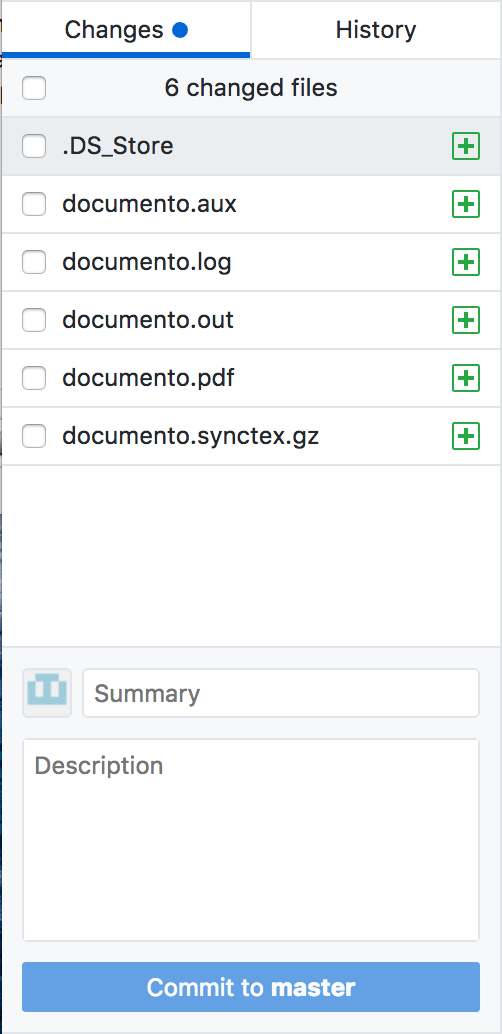
\includegraphics[width=\textwidth]{Figuras/cambios2.png}
        \caption{Después de \texttt{commit}.}
        \label{cambios2}
    \end{subfigure}
    ~ %add desired spacing between images, e. g. ~, \quad, \qquad, \hfill etc. 
    %(or a blank line to force the subfigure onto a new line)
    \caption{Cambios y \texttt{commit}.}\label{cambios}
\end{figure}

Para publicar el repositorio e incluir los cambios realizados a GitHub online, se debe seleccionar el botón \textbf{Publish repository} (Figura \ref{pure1}). Se debe incluir un nombre, descripción y deseleccionar la opción \textit{Keep this code private}, ya que es una opción válida sólo para cuentas de pago (Figura \ref{pure2}).\\

\begin{figure}[!h]
    \centering
    \begin{subfigure}[b]{0.25\textwidth}
        
\includegraphics[width=\textwidth]{Figuras/pure1.png}
        \caption{Botón para publicar repositorio.}
        \label{pure1}
    \end{subfigure}
    ~ %add desired spacing between images, e. g. ~, \quad, \qquad, \hfill etc. 
      %(or a blank line to force the subfigure onto a new line)
    \begin{subfigure}[b]{0.5\textwidth}
        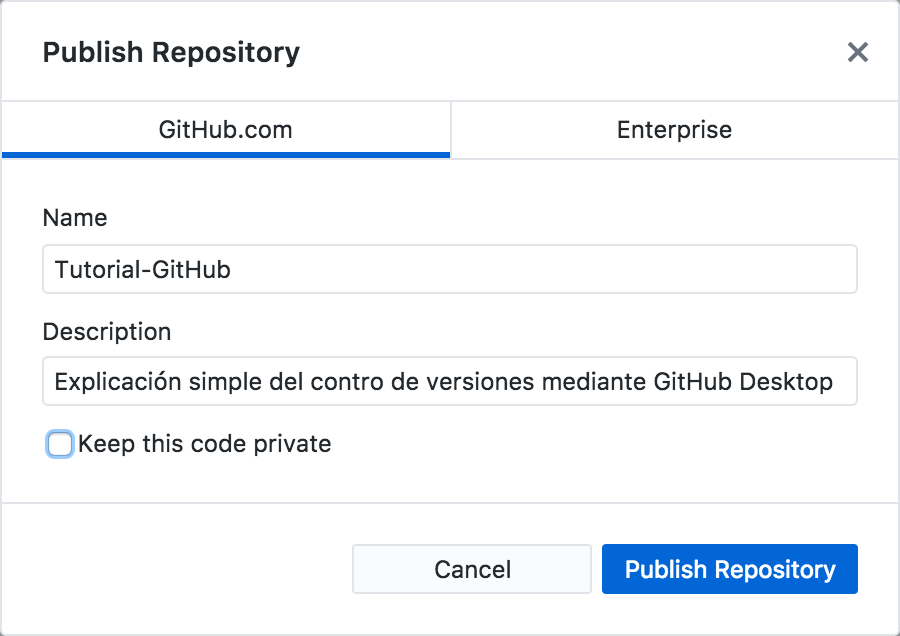
\includegraphics[width=\textwidth]{Figuras/pure2.png}
        \caption{Opciones de publicación.}
        \label{pure2}
    \end{subfigure}
    ~ %add desired spacing between images, e. g. ~, \quad, \qquad, \hfill etc. 
    %(or a blank line to force the subfigure onto a new line)
    \caption{Publicación de repositorio.}\label{pure}
\end{figure}

Una vez actualizada la versión web, la cargará el repositorio a GitHub online a la web de la forma \verb+https://github.com/nombre_usuario/nombre_repositorio+. Para este caso, \url{https://github.com/aldotapia/Tutorial-GitHub} (Figura \ref{web2}).\\

\begin{figure}[!h]
  \centering
    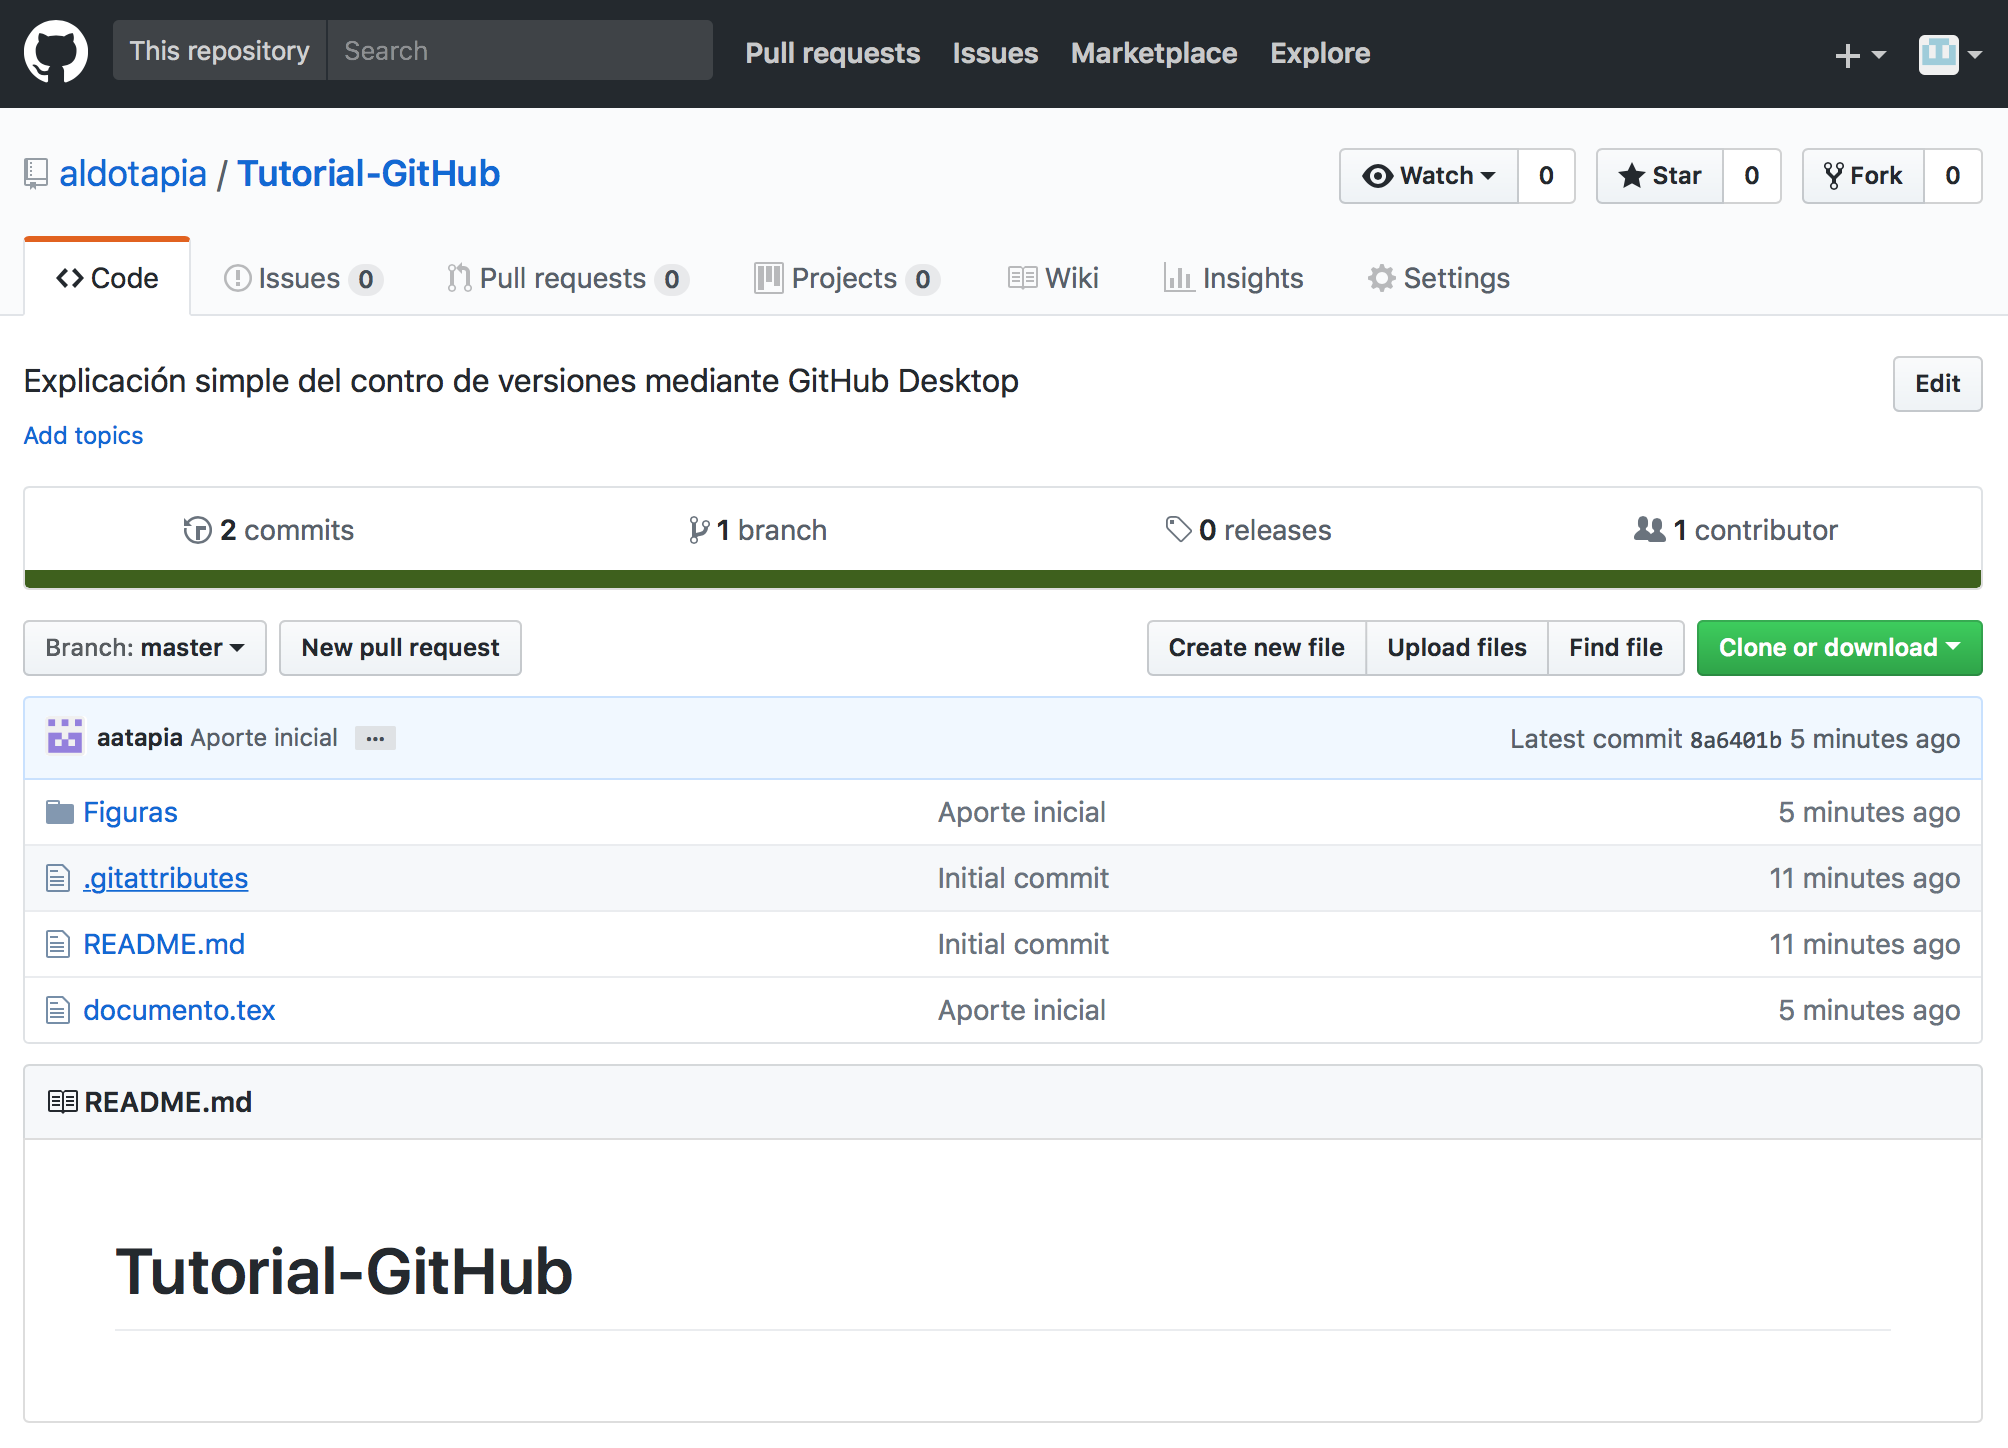
\includegraphics[width=0.5\textwidth]{Figuras/web2.png}
  \caption{Versión web GitHub Desktop.}
  \label{web2}
\end{figure}

\FloatBarrier

\section{Ignorando archivos}

Tal como se mencionó en párrafos anteriores, muchos archivos dentro de la carpeta de trabajo pueden no ser necesarios subir al repositorio. Para dejarlos fuera de manera eficiente (para no deseleccionarlos en cada \texttt{Commit}, clickearlos con el botón derecho y seleccionar \textbf{Ignore} (Figura \ref{ignore1}). Esto creará un archivo denominado \texttt{.gitignore} con los nombres de los archivos a ignorar en cada \texttt{Commit}.\\

\begin{figure}[!h]
    \centering
    \begin{subfigure}[b]{0.25\textwidth}
        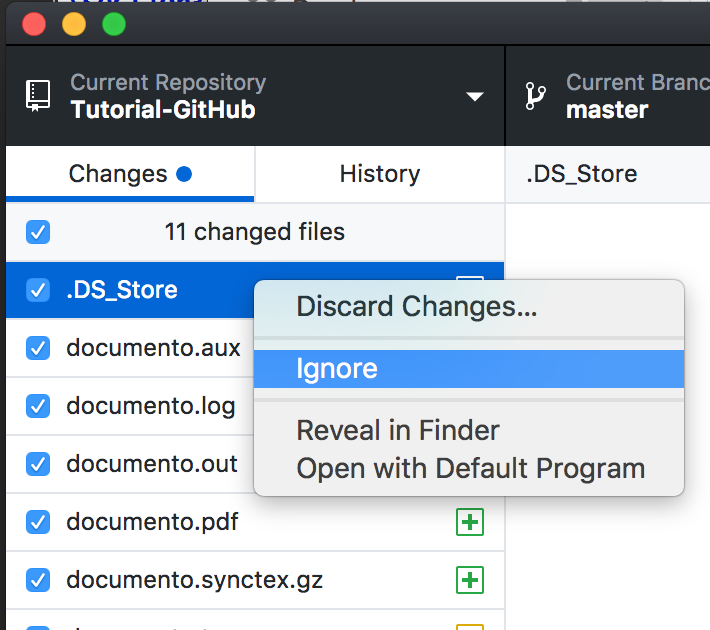
\includegraphics[width=\textwidth]{Figuras/ignorar1.png}
        \caption{\textbf{Ignore} en menú.}
        \label{ignore1}
    \end{subfigure}
    ~ %add desired spacing between images, e. g. ~, \quad, \qquad, \hfill etc. 
      %(or a blank line to force the subfigure onto a new line)
    \begin{subfigure}[b]{0.5\textwidth}
        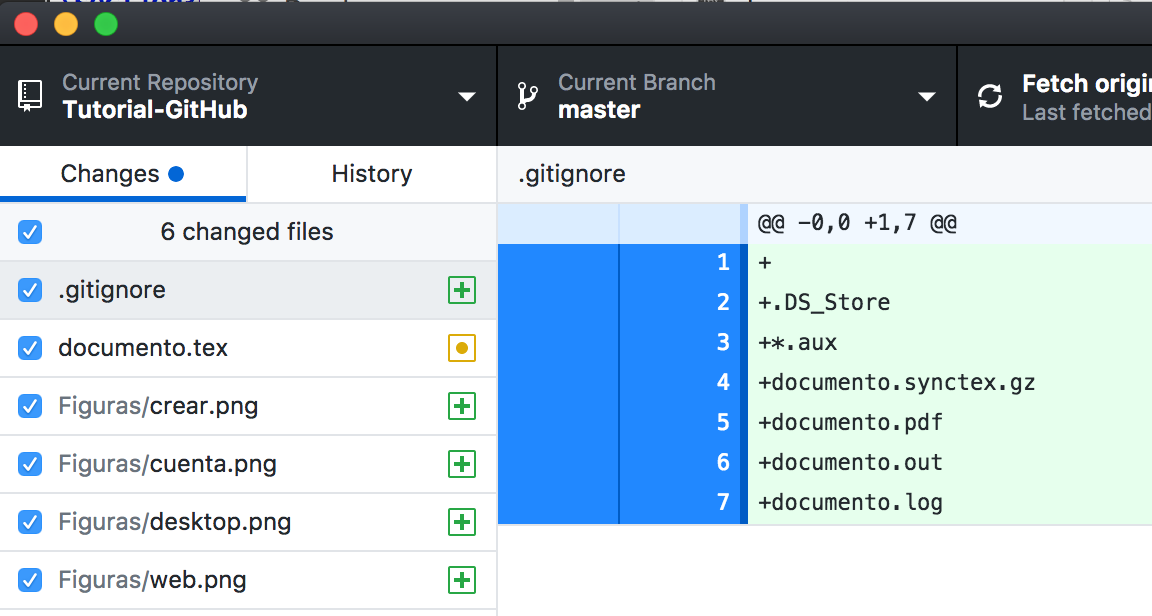
\includegraphics[width=\textwidth]{Figuras/ignorar2.png}
        \caption{contenido \texttt{.gitignore}.}
        \label{ignore2}
    \end{subfigure}
    ~ %add desired spacing between images, e. g. ~, \quad, \qquad, \hfill etc. 
    %(or a blank line to force the subfigure onto a new line)
    \caption{Ignorando archivos dentro del repositorio.}\label{ignore}
\end{figure}

\end{document}